\documentclass[12pt,a4paper]{article}
%\usepackage{ctex}
\usepackage{amsmath,amscd,amsbsy,amssymb,latexsym,url,bm,amsthm}
\usepackage{epsfig,graphicx,subfigure}
\usepackage{enumitem,balance}
\usepackage{wrapfig}
\usepackage{mathrsfs, euscript}
\usepackage[usenames]{xcolor}
\usepackage{hyperref}
\usepackage[vlined,ruled,commentsnumbered,linesnumbered]{algorithm2e}
\usepackage{ulem}
\usepackage{url}

\newtheorem{theorem}{Theorem}[section]
\newtheorem{lemma}[theorem]{Lemma}
\newtheorem{proposition}[theorem]{Proposition}
\newtheorem{corollary}[theorem]{Corollary}
\newtheorem{exercise}{Exercise}[section]
\newtheorem*{solution}{Solution}
\theoremstyle{definition}


\numberwithin{equation}{section}
\numberwithin{figure}{section}

\renewcommand{\thefootnote}{\fnsymbol{footnote}}

\newcommand{\postscript}[2]
 {\setlength{\epsfxsize}{#2\hsize}
  \centerline{\epsfbox{#1}}}

\renewcommand{\baselinestretch}{1.0}

\setlength{\oddsidemargin}{-0.365in}
\setlength{\evensidemargin}{-0.365in}
\setlength{\topmargin}{-0.3in}
\setlength{\headheight}{0in}
\setlength{\headsep}{0in}
\setlength{\textheight}{10.1in}
\setlength{\textwidth}{7in}
\makeatletter \renewenvironment{proof}[1][Proof] {\par\pushQED{\qed}\normalfont\topsep6\p@\@plus6\p@\relax\trivlist\item[\hskip\labelsep\bfseries#1\@addpunct{.}]\ignorespaces}{\popQED\endtrivlist\@endpefalse} \makeatother
\makeatletter
\renewenvironment{solution}[1][Solution] {\par\pushQED{\qed}\normalfont\topsep6\p@\@plus6\p@\relax\trivlist\item[\hskip\labelsep\bfseries#1\@addpunct{.}]\ignorespaces}{\popQED\endtrivlist\@endpefalse} \makeatother



\begin{document}
\noindent

%========================================================================
\noindent\framebox[\linewidth]{\shortstack[c]{
\Large{\textbf{Computer Graphics Assignment 2}}}}
\begin{center}

\footnotesize{\color{blue}$*$ Name:Yongxi Huang  \quad Student ID:119033910011 \quad Email: huangyongxi@sjtu.edu.cn}
\end{center}

\noindent\textbf{Code will be uploaded to \\
	\url{https://github.com/Riften/SJTU-Computer-Graphics-2020-Assignments}\\
	 after deadline.}

\section{Question 1}
\subsection{Result}
\begin{figure}[htbp]
	\centering
	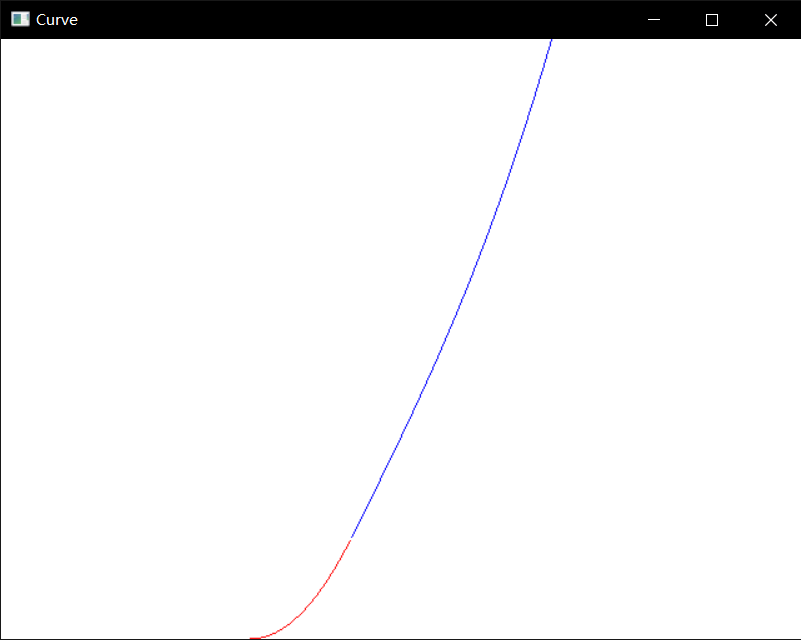
\includegraphics[width=0.5\linewidth]{curve1.png}
	\caption{Curves for question 1.}
	\label{fig1}
\end{figure}
Two curves are shown in Fig.\ref{fig1}. The red curve is $\gamma(t)$ and the blue one is $\eta(t)$. These two curves intersect at $(1,1)$ and have the same tangent vector $(1,2)$ at that point. So they meet both $C^1$ and $G^1$ continuity at the intersection.

\subsection{Implementation}
In order to draw these curves, I implement several classes to define and draw any cubic functions. The major classes are
\begin{enumerate}
	\item \textbf{CubicFunc}: Represents a cubic function. It contains 4 coefficients and the domain of definition.
	\item \textbf{CubicCurve}: Each CubicCurve contains two CubicFunc, $x(t)$ and $y(t)$. CubicCurve can compute several coordinates based on domain of t and an interval.
	\item \textbf{CurveCache}: CurveCache is used to save the coordinates computed by CubicCurve. With a CurveCache, we can draw a curve by connecting the coordinates using line strips. CurveCache.draw() also design the method to resize the coordinates so that we can draw it properly on the canvas.
	\item \textbf{CurveDrawer}: Used to draw a list of curves according to a list of CurveCache.
\end{enumerate}

The drawing method is simple. Given a list coordinates, the curve is drawed by connecting them using line strips. Please refer to the source code for more details.
\section{Question 2}
\subsection{Compute $B_{0,4}$}
$t_0=0$, $t_1=1$, $t_2=3$, $t_3=4$, $t_4=5$

The recursive formula of $B_{i,deg}$ is

\begin{align*}
B_{i,1}(t)&=\left\{
\begin{array}{lr}
1,~t_i\leq t \leq t_{i+1}\\
0,~otherwise
\end{array}
\right.\\
B_{i,2}(t) &= \frac{t-t_i}{t_{i+1}-t_i}B_{i,1}(t)+\frac{t_{i+2}-t}{t_{i+2}-t_{i+1}}B_{i+1,1}(t)\\
B_{i,3}(t) &= \frac{t-t_i}{t_{i+2}-t_i}B_{i,2}(t)+\frac{t_{i+3}-t}{t_{i+3}-t_{i+1}}B_{i+1,2}(t)\\
B_{i,4}(t) &= \frac{t-t_i}{t_{i+3}-t_i}B_{i,3}(t)+\frac{t_{i+4}-t}{t_{i+4}-t_{i+1}}B_{i+1,3}(t)
\end{align*}
According to the recursive formula, we get
\begin{align*}
B_{0,2}&= \frac{t-t_0}{t_{1}-t_0}B_{0,1}(t)+\frac{t_{2}-t}{t_{2}-t_{1}}B_{1,1}(t)\\
&=tB_{0,1}(t)+\frac{3-t}{2}B_{1,1}(t)\\
&=\left\{
\begin{array}{lr}
t, ~~~~~0\leq t< 1\\
\frac{3-t}{2}, ~~1\leq t<3\\
0,~~~otherwise
\end{array}
\right.\\
\end{align*}
\begin{align*}
%============================================
B_{1,2}&= \frac{t-t_1}{t_{2}-t_1}B_{1,1}(t)+\frac{t_{3}-t}{t_{3}-t_{2}}B_{2,1}(t)\\
&=\frac{t-1}{2}B_{1,1}(t)+(4-t)B_{2,1}(t)\\
&=\left\{
\begin{array}{lr}
\frac{t-1}{2}, ~~~~1\leq t< 3\\
4-t, ~~3\leq t<4\\
0,~~~otherwise
\end{array}
\right.\\
\end{align*}
\begin{align*}
%=============================================
B_{2,2}&= \frac{t-t_2}{t_{3}-t_2}B_{2,1}(t)+\frac{t_{4}-t}{t_{4}-t_{3}}B_{3,1}(t)\\
&=(t-3)B_{2,1}(t)+(5-t)B_{3,1}(t)\\
&=\left\{
\begin{array}{lr}
t-3, ~~~3\leq t< 4\\
5-t, ~~4\leq t<5\\
0,~~~otherwise
\end{array}
\right.\\
\end{align*}
\begin{align*}
%==============================================
B_{0,3}&= \frac{t-t_0}{t_{2}-t_0}B_{0,2}(t)+\frac{t_{3}-t}{t_{3}-t_{1}}B_{1,2}(t)\\
&=\frac{t}{3}B_{0,2}(t)+\frac{4-t}{3}B_{1,2}(t)\\
&=\left\{
\begin{array}{lr}
\frac{t^2}{3}, ~~0\leq t< 1\\
\frac{-t^2+4t-2}{3}, ~~1\leq t<3\\
\frac{t^2-8t+16}{3}, ~~3\leq t<4\\
0,~~~otherwise
\end{array}
\right.\\
\end{align*}
\begin{align*}
%=================================================
B_{1,3}&= \frac{t-t_1}{t_{3}-t_1}B_{1,2}(t)+\frac{t_{4}-t}{t_{4}-t_{2}}B_{2,2}(t)\\
&=\frac{t-1}{3}B_{1,2}(t)+\frac{5-t}{2}B_{2,2}(t)\\
&=\left\{
\begin{array}{lr}
\frac{(t-1)^2}{6}, ~~1\leq t< 3\\
\frac{-5t^2+34t-53}{6}, ~~3\leq t<4\\
\frac{(5-t)^2}{2}, ~~4\leq t<5\\
0,~~~otherwise
\end{array}
\right.\\
\end{align*}
\begin{align*}
%==================================================
B_{0,4}&= \frac{t-t_0}{t_{3}-t_0}B_{0,3}(t)+\frac{t_{4}-t}{t_{4}-t_{1}}B_{1,3}(t)\\
&=\frac{t}{4}B_{0,3}(t)+\frac{5-t}{4}B_{1,3}(t)\\
&=\left\{
\begin{array}{lr}
\frac{t^3}{12}, ~~0\leq t< 1\\
\frac{-3t^3+15t^2-15t+5}{24}, ~~1\leq t< 3\\
\frac{7t^3-75t^2+255t-265}{24}, ~~3\leq t<4\\
\frac{(5-t)^3}{8}, ~~4\leq t<5\\
0,~~~otherwise
\end{array}
\right.\\
\end{align*}
\begin{figure}[p]
	\centering
	\subfigure[B01]{
		\label{figb01}
		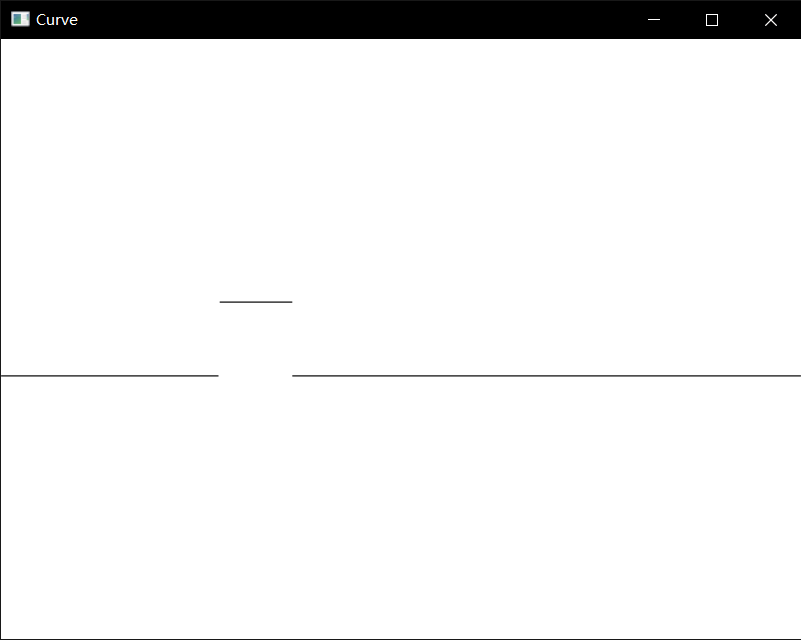
\includegraphics[width=0.27\linewidth]{B01.png}
	}
	\quad
	\subfigure[B11]{
		\label{figb11}
		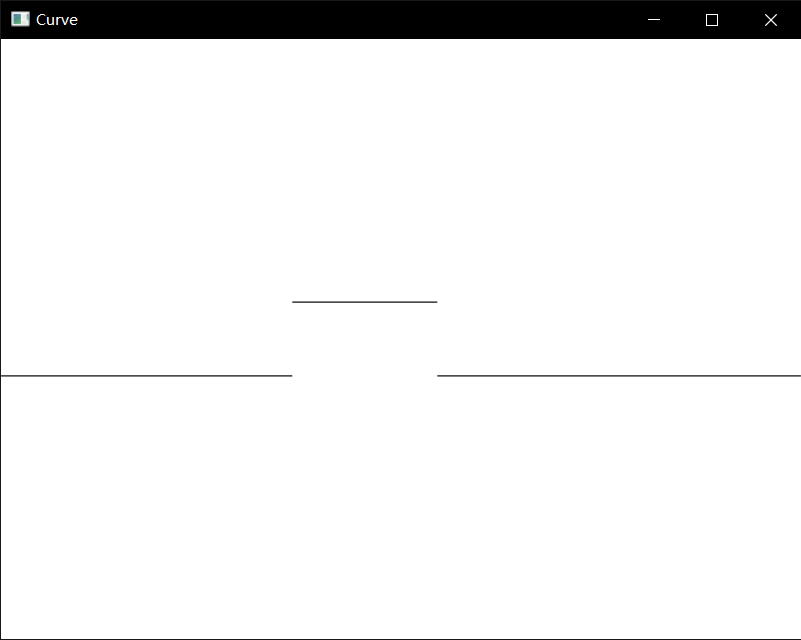
\includegraphics[width=0.27\linewidth]{B11.png}
	}
	\quad
	\subfigure[B21]{
		\label{figb21}
		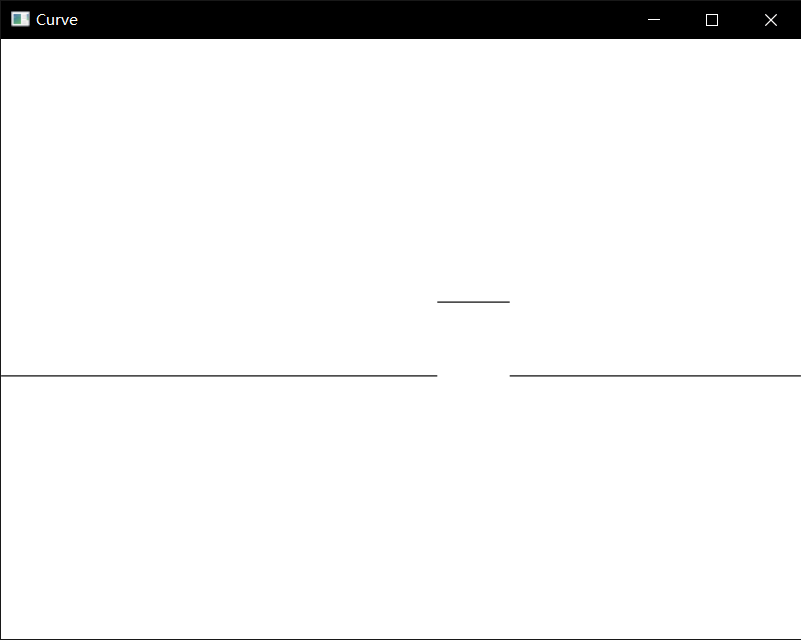
\includegraphics[width=0.27\linewidth]{B21.png}
	}
	\quad
	\subfigure[B31]{
		\label{figb31}
		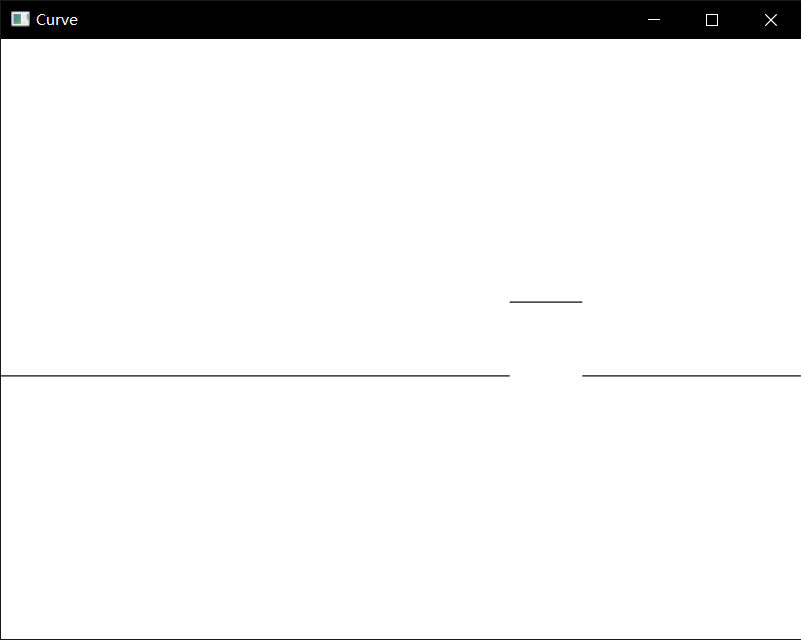
\includegraphics[width=0.27\linewidth]{B31.png}
	}
	\quad
	\subfigure[B02]{
		\label{figb02}
		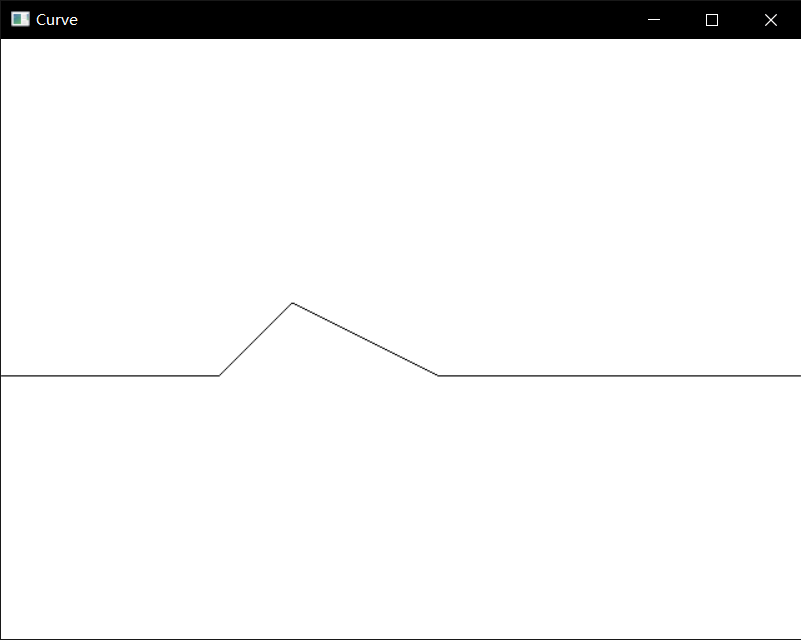
\includegraphics[width=0.27\linewidth]{B02.png}
	}
	\quad
	\subfigure[B12]{
		\label{figb12}
		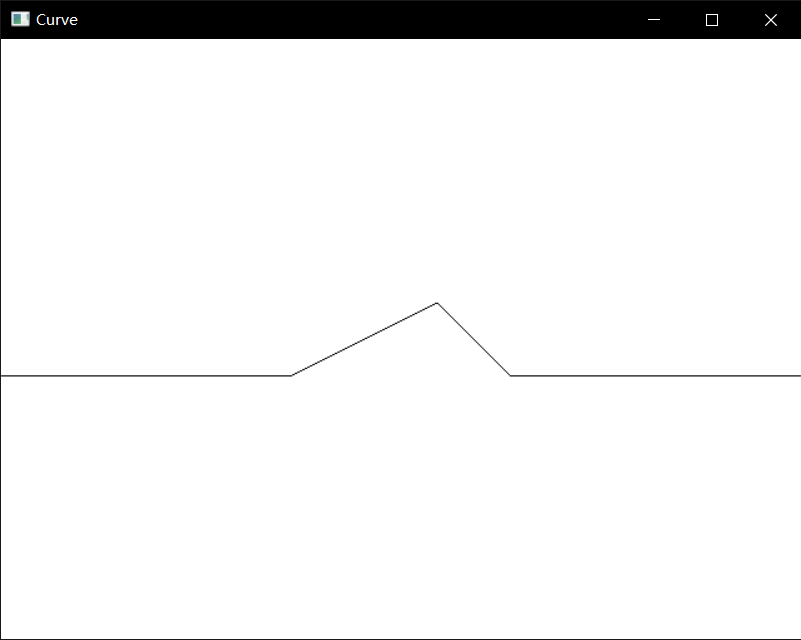
\includegraphics[width=0.27\linewidth]{B12.png}
	}
	\quad
	\subfigure[B22]{
		\label{figb22}
		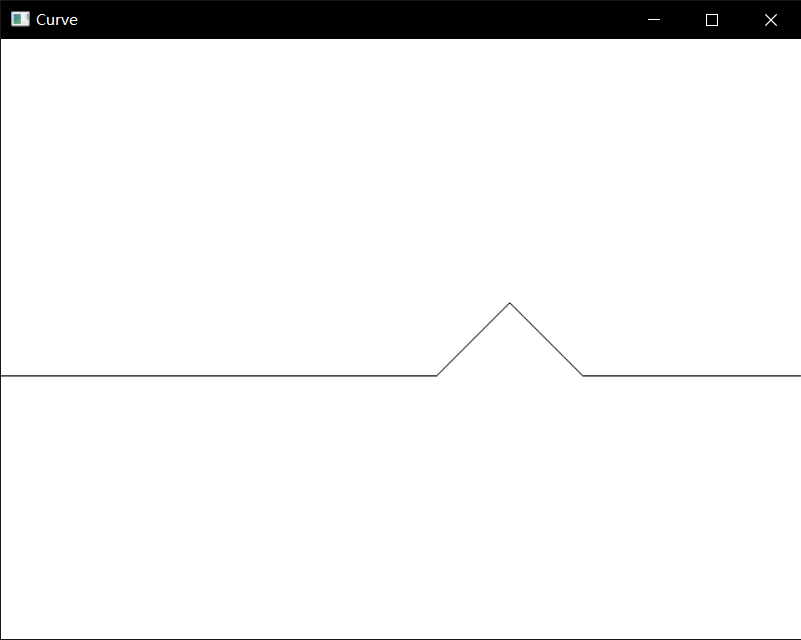
\includegraphics[width=0.27\linewidth]{B22.png}
	}
	\quad
	\subfigure[B03]{
		\label{figb03}
		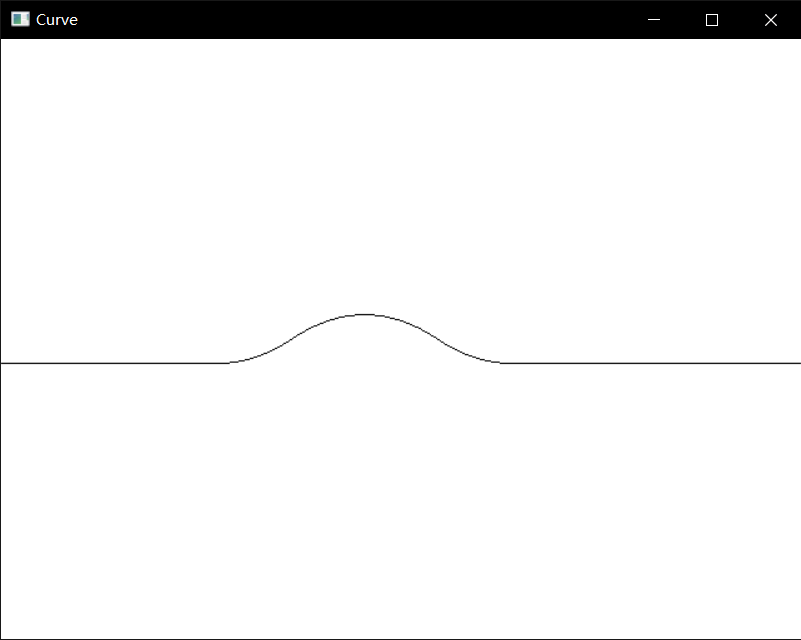
\includegraphics[width=0.27\linewidth]{B03.png}
	}
	\quad
	\subfigure[B13]{
		\label{figb13}
		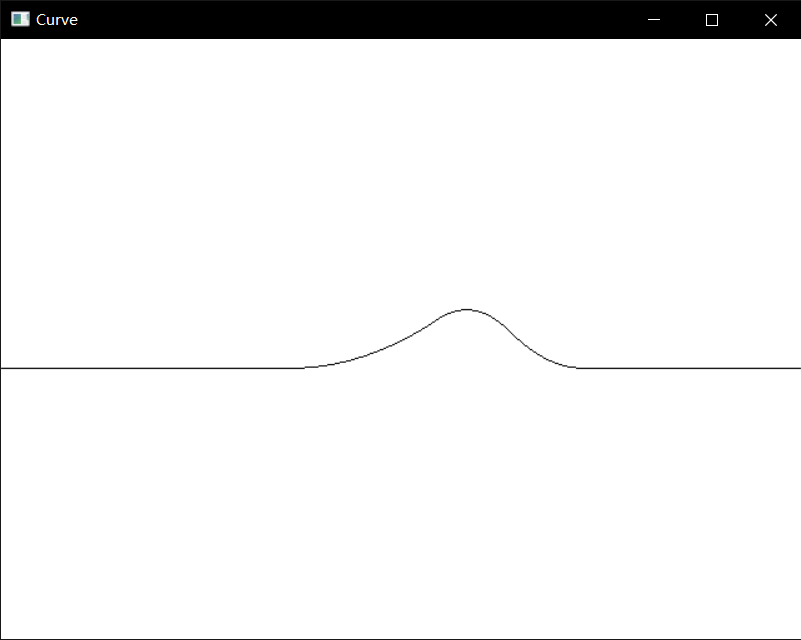
\includegraphics[width=0.27\linewidth]{B13.png}
	}
	\quad
	\subfigure[B04]{
		\label{figb04}
		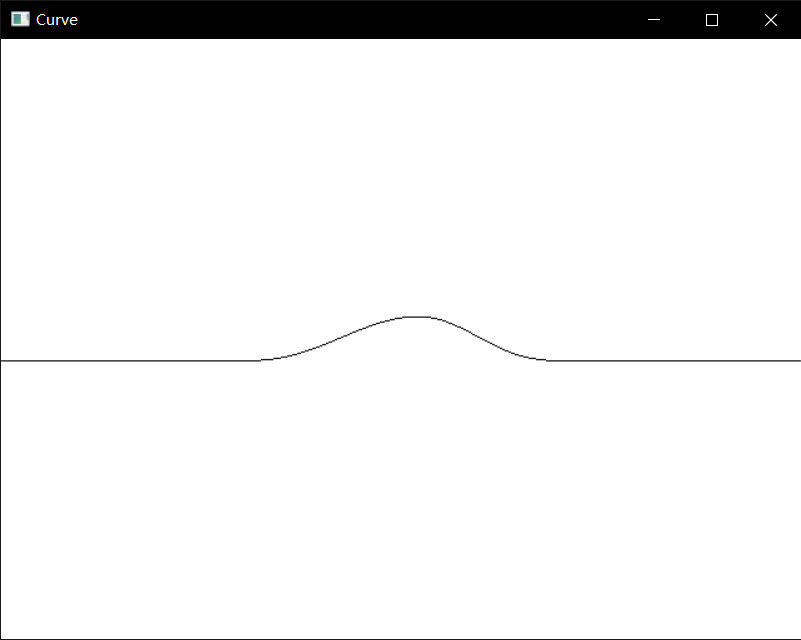
\includegraphics[width=0.27\linewidth]{B04.png}
	}
	\caption{Curves for question 2}
	\label{fig2}
\end{figure}
Then we try to plot these functions on the interval $-3\leq t \leq 8$. It would be easy to use the toolkit built in question 1 to plot these functions. However, here I use a \textbf{recursive method} to draw these functions. That is because we only need the function value of some specific $t$ instead of the whole formula to plot a function.

A new class \textbf{BCurve} is implemented to compute and draw B functions. It will recursively compute the function value at each $t$ selected according to a interval. A \textbf{CurveCache} mentioned in question 1 is used to save the result and draw curves. Please refer to the source code for more details.

The functions plotted by recursive method is shown in Fig.\ref{fig2}.


%\bibliography{ref}{}
%\bibliographystyle{IEEEtran}
%========================================================================
\end{document}
